\documentclass[aspectratio=169]{beamer}

\usepackage{listings}
\usepackage{color}
\definecolor{dkgreen}{rgb}{0,0.6,0}
\definecolor{gray}{rgb}{0.5,0.5,0.5}
\definecolor{mauve}{rgb}{0.58,0,0.82}

\usepackage{graphicx}
\usepackage{tikz}
\usetikzlibrary{matrix,fit,positioning,overlay-beamer-styles}
\usetikzlibrary{shapes.multipart}

\lstdefinestyle{myScalastyle}{
  language=scala,
  aboveskip=2mm,
  belowskip=2mm,
  showstringspaces=false,
  columns=flexible,
  basicstyle={\small\ttfamily},
  numbers=none,
  numberstyle=\small\color{gray},
  keywordstyle=\color{blue},
  commentstyle=\color{dkgreen},
  stringstyle=\color{mauve},
  frame=single,
  breaklines=true,
  breakatwhitespace=true,
  tabsize=3,
}

\beamertemplatenavigationsymbolsempty

\title{Extreme deduplication}
\author{Vincent de Haan}
\date{}


\begin{document}

\begin{frame}
\maketitle

\center{https://github.com/vincentdehaan/extreme-deduplication}
\end{frame}

\begin{frame}
\begin{columns}
\begin{column}{0.4\textwidth}

\includegraphics[width=\textwidth]{the-pragmatic-programmer-from-journeyman-to-master-1.jpg}
\end{column}
\pause
\begin{column}{0.6\textwidth}
"Every piece of knowledge must have a single, unambiguous, authoritative representation within a system." (p. 27)
\end{column}
\end{columns}
\end{frame}

\begin{frame}
\frametitle{What are we going to do today?}

\begin{itemize}
\item Build a simple HTTP application
\pause
\item \ldots with OpenAPI documentation
\item \ldots with a TypeScript frontend
\item \ldots with a DynamoDB database
\pause
\item \ldots with every piece of knowledge stored in a single, unambiguous, autoritative representation.
\end{itemize}

\end{frame}

\begin{frame}[fragile]
  \frametitle{OpenAPI documentation}
1st idea: generate the code from the docs

\hfill \break

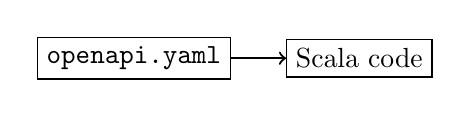
\begin{tikzpicture}
  \matrix [row sep=3em,
    column sep=2em]{
    \node (src1) [draw, shape=rectangle] {\texttt{openapi.yaml}}; &
  \node (dst1) [draw, shape=rectangle] {Scala code};\\};
  \draw[->, thick] (src1) -- (dst1);
\end{tikzpicture}
\pause

\hfill \break
2nd idea: generate the docs from the code

\hfil \break

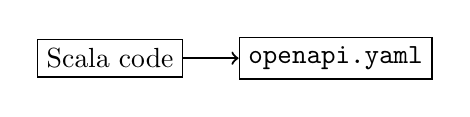
\begin{tikzpicture}
  \matrix [row sep=3em,
    column sep=2em]{
    \node (src1) [draw, shape=rectangle] {Scala code}; &
  \node (dst1) [draw, shape=rectangle] {\texttt{openapi.yaml}};\\};
  \draw[->, thick] (src1) -- (dst1);
\end{tikzpicture}
\end{frame}

\begin{frame}[fragile]
  \frametitle{OpenAPI documentation}
Generate the code and the docs from an intermediate representation

\hfill \break

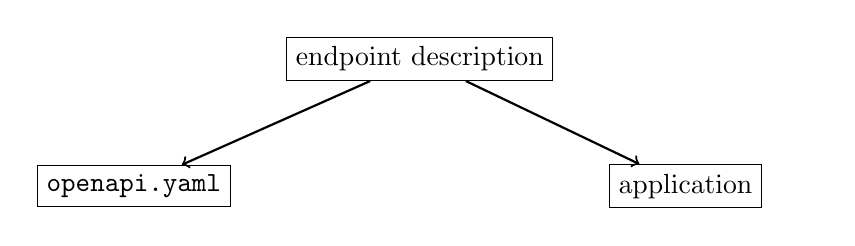
\begin{tikzpicture}
  \matrix [row sep=3em,
    column sep=2em]{
  &  \node (src1) [draw, shape=rectangle] {endpoint description}; \\
  \node (dst1) [draw, shape=rectangle] {\texttt{openapi.yaml}}; &&
  \node (dst2) [draw, shape=rectangle] {application}; &\\};
  \draw[->, thick] (src1) -- (dst1);
\draw[->, thick] (src1) -- (dst2);
\end{tikzpicture}

\end{frame}

\begin{frame}[fragile]
  \frametitle{Use tapir}
build.sbt:
\begin{lstlisting}[style=myScalaStyle,frame=none]
libraryDependencies += "com.softwaremill.sttp.tapir" %% "tapir-core" % tapirVersion
\end{lstlisting}
\pause
\begin{columns}
\begin{column}{0.4\textwidth}
\begin{lstlisting}[style=myScalaStyle,frame=none]
POST /foo
Content-Type: application/json
{
  "name": "foo's name", 
  "id": 1,
  "description":"foo's description"
}
\end{lstlisting}
\end{column}
\pause
\begin{column}{0.6\textwidth}
Api.scala:
\begin{lstlisting}[style=myScalaStyle,frame=none]
class Api(service: Service){
  val endpoints = List(
    endpoint
      .post
      .in("foo")
      .in(jsonBody[Foo])
      .out(statusCode(StatusCode.Accepted))
      .description("Use this endpoint to create a foo")
      .serverLogic(service.createFoo)
  )
}

\end{lstlisting}
\end{column}
\end{columns}

\end{frame}

\begin{frame}[fragile]
Interpret endpoint definition as documentation:

\frametitle{Use tapir}
\begin{lstlisting}[style=myScalaStyle,frame=none,numbers=left]
object DocWriter extends App with OpenAPIDocsInterpreter {
  val endpointList: List[AnyEndpoint] =
    new Api(null).endpoints.map(_.endpoint)
  val docs = toOpenAPI(endpointList, "My App", "1.0")
    .copy(servers = List(Server("http://localhost:8080")))
  val filePath = new File("target/openapi/openapi.yaml")
  filePath.getParentFile.mkdirs()
  val printWriter = new PrintWriter(filePath)
  printWriter.print(docs.toYaml)
  printWriter.close()
}

\end{lstlisting}


\end{frame}

\begin{frame}[fragile]

\frametitle{Use tapir}
Interpret endpoint definition as HTTP server:

\begin{lstlisting}[style=myScalaStyle,frame=none,numbers=left]
object Main extends App {
  implicit val system = ActorSystem("my-system")
  implicit val executionContext = system.dispatcher
  val service = new ServiceImpl()
  val api = new Api(service)

  val bindingFuture = Http().newServerAt("0.0.0.0", 8080).bind(
    AkkaHttpServerInterpreter().toRoute(api.endpoints))

  StdIn.readLine()
}
\end{lstlisting}
\end{frame}

\begin{frame}[fragile]
\frametitle{Sbt project structure}

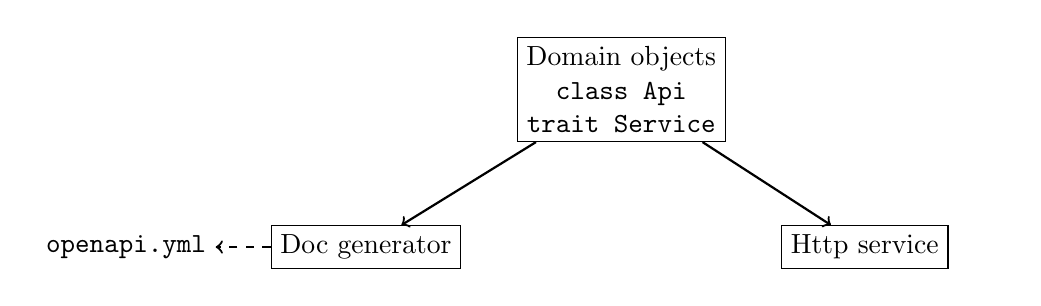
\begin{tikzpicture}[every text node part/.style={align=center}]
  \matrix [row sep=3em,
    column sep=2em]{
  &&  \node (src1) [draw, shape=rectangle] {Domain objects \\ \texttt{class Api} \\ \texttt{trait Service}}; \\
  \node (doc) [draw=none] {\texttt{openapi.yml}}; &
  \node (dst1) [draw, shape=rectangle] {Doc generator}; &&
  \node (dst2) [draw, shape=rectangle] {Http service}; &\\};
  \draw[->, thick] (src1) -- (dst1);
\draw[->, thick] (src1) -- (dst2);
\draw[->,thick,dashed] (dst1) -- (doc);
\end{tikzpicture}

\end{frame}

\begin{frame}[fragile]
\frametitle{Generate TypeScript interfaces}

\begin{columns}
\begin{column}{0.4\textwidth}
\begin{lstlisting}[style=myScalaStyle,frame=none]
case class Foo(
  name: String,
  id: Int,
  description: String
)

case class Bar(
  barName: String, 
  barId: Int
)
\end{lstlisting}
\end{column}
\begin{column}{0.4\textwidth}
\begin{lstlisting}[style=myScalaStyle,frame=none]
export interface IFoo {
  name: string
  id: number
  description: string
}

export interface IBar {
  barName: string
  barId: number
}
\end{lstlisting}
\end{column}
\end{columns}
\end{frame}

\begin{frame}[fragile]
\frametitle{Use scala-tsi}

plugins.sbt:
\begin{lstlisting}[style=myScalaStyle,frame=none]
addSbtPlugin("com.scalatsi" % "sbt-scala-tsi" % "0.8.2")
\end{lstlisting}
\pause
build.sbt:
\begin{lstlisting}[style=myScalaStyle,frame=none, numbers=left,escapeinside=||]
lazy val domain = (project in file("domain")) |\pause|
  .enablePlugins(ScalaTsiPlugin) |\pause|
  .settings(
    typescriptExports :=  |\only<4>{Seq("Foo", "Bar),}| |\pause|
      Source.fromInputStream(
        java.lang.Runtime.getRuntime.exec("find domain/src/main/scala/ -type f -exec cat {} +").getInputStream
      ).getLines().flatMap(l => 
        """case class ([a-zA-Z]+)""".r.findFirstMatchIn(l).map(
          _.subgroups(0))).toSeq, |\pause|
    typescriptOutputFile := baseDirectory.value / "target/index.d.ts",
    typescriptGenerationImports := Seq("nl.vindh.extdup.domain._")
  )

\end{lstlisting}

\end{frame}

\begin{frame}[fragile]
\frametitle{Sbt project structure}

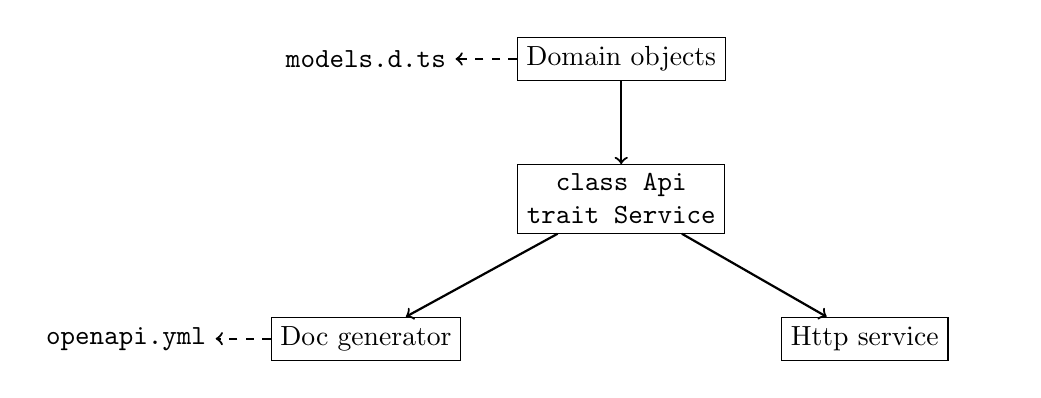
\begin{tikzpicture}[every text node part/.style={align=center}]
  \matrix [row sep=3em,
    column sep=2em]{
 & \node (ts) [draw=none] {\texttt{models.d.ts}};
 & \node (src0) [draw, shape=rectangle] {Domain objects}; \\
  &&  \node (src1) [draw, shape=rectangle] {\texttt{class Api} \\ \texttt{trait Service}}; \\
  \node (doc) [draw=none] {\texttt{openapi.yml}}; &
  \node (dst1) [draw, shape=rectangle] {Doc generator}; &&
  \node (dst2) [draw, shape=rectangle] {Http service}; &\\};
  \draw[->, thick] (src1) -- (dst1);
\draw[->, thick] (src1) -- (dst2);
\draw[->, thick] (src0) -- (src1);
\draw[->,thick,dashed] (dst1) -- (doc);
\draw[->, thick, dashed] (src0) -- (ts);
\end{tikzpicture}
\end{frame}

\begin{frame}
\frametitle{Database requirements}

\begin{enumerate}
\item I can only create a \texttt{Repository[T]} if a table for objects of type \texttt{T} exists \only<2>{ in the infrastructure code}.
\item I can only create an index for a field \texttt{f} if \texttt{f} is a field of type \texttt{T}.
\item I can only create a query on an index if that index exists in the database.


\end{enumerate}

\end{frame}

\begin{frame}[fragile]
\frametitle{Database requirement 1}
I can only create a \texttt{Repository[T]} if a table for objects of type \texttt{T} exists in the infrastructure code.
\hfill \break

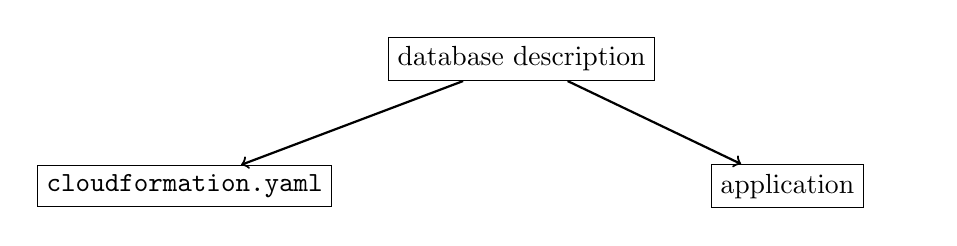
\begin{tikzpicture}
  \matrix [row sep=3em,
    column sep=2em]{
  &  \node (src1) [draw, shape=rectangle] {database description}; \\
  \node (dst1) [draw, shape=rectangle] {\texttt{cloudformation.yaml}}; &&
  \node (dst2) [draw, shape=rectangle] {application}; &\\};
  \draw[->, thick] (src1) -- (dst1);
\draw[->, thick] (src1) -- (dst2);
\end{tikzpicture}
\end{frame}

\begin{frame}[fragile]
\frametitle{Database requirement 1}
I can only create a \texttt{Repository[T]} if a table for objects of type \texttt{T} exists in the infrastructure code.
\hfill \break
\begin{lstlisting}[style=myScalaStyle,frame=none,escapeinside=||]

case class Table(name: String)
|\pause|
val Tables = Seq(
  Table("Foo")
)

\end{lstlisting}

\end{frame}

\begin{frame}[fragile]
\frametitle{Database requirement 1}
I can only create a \texttt{Repository[T]} if a table for objects of type \texttt{T} exists in the infrastructure code.
\hfill \break
\begin{lstlisting}[style=myScalaStyle,frame=none,escapeinside=||,numbers=left]
object Table {
  def create[T : Typeable] = TypedTable[T](())
}

case class TypedTable[T : Typeable](u: Unit)
  
 

\end{lstlisting}

\end{frame}

\begin{frame}[fragile]
\frametitle{Database requirement 1}
I can only create a \texttt{Repository[T]} if a table for objects of type \texttt{T} exists in the infrastructure code.
\hfill \break
\begin{lstlisting}[style=myScalaStyle,frame=none,escapeinside=||,numbers=left]
case class Foo(name: String, id: Int, description: String)
case class Bar(barName: String, barId: Int)

val tables =
  Table.create[Foo] ::
  Table.create[Bar] :: HNil

\end{lstlisting}

\end{frame}

\begin{frame}[fragile]
\frametitle{Database requirement 1}
I can only create a \texttt{Repository[T]} if a table for objects of type \texttt{T} exists in the infrastructure code.
\hfill \break
\begin{lstlisting}[style=myScalaStyle,frame=none,escapeinside=||,numbers=left]
abstract class Repository[T: DynamoFormat] {
  protected val tableInfo: TableInfo[T]

  object tableSelector extends Poly1 {
    implicit def thisCase[H <: HList] = at[TypedTable[T, H]](_ :: HNil)
    implicit def otherCase[U, H <: HList](implicit ev: U =:!= T) = at[TypedTable[U, H]](_ => HNil)
  }
}
|\pause|
class FooRepository extends Repository[Foo] {
  val tableInfo: TableInfo[Foo] = Tables.tables.flatMap(tableSelector).head.toTableInfo
}

\end{lstlisting}

\end{frame}


\begin{frame}[fragile]
\frametitle{Database requirement 2}
I can only create an index for a field \texttt{f} if \texttt{f} is a field of type \texttt{T}.
\hfill \break
\begin{lstlisting}[style=myScalaStyle,frame=none,escapeinside=||]
case class Foo(name: String, id: Int, description: String)

case class Table[T](indices: Seq[String])

val Tables = Seq(
  Table[Foo](Seq("name"))
)

\end{lstlisting}

\end{frame}

\begin{frame}[fragile]
\frametitle{Database requirement 2}
I can only create an index for a field \texttt{f} if \texttt{f} is a field of type \texttt{T}.
\hfill \break
\begin{lstlisting}[style=myScalaStyle,frame=none,escapeinside=||,numbers=left]
object Table {
  def create[T : Typeable] = TypedTable[T, HNil](Seq())
}

case class TypedTable[T : Typeable, I <: HList] 
  private(indices: Seq[String]) {
    def withIndex[L <: HList, S](idx: Witness)(implicit 
      gen: LabelledGeneric.Aux[T, L], 
      selector: Selector.Aux[L, idx.T, S], 
      ev: S =:= String
    ): TypedTable[T, idx.T :: I] =
      TypedTable(indices :+ idx.value.asInstanceOf[Symbol].name)
  }

\end{lstlisting}

\end{frame}

\begin{frame}[fragile]
\frametitle{Database requirement 2}
I can only create an index for a field \texttt{f} if \texttt{f} is a field of type \texttt{T}.
\hfill \break
\begin{lstlisting}[style=myScalaStyle,frame=none,escapeinside=||,numbers=left]
case class Foo(name: String, id: Int, description: String)
case class Bar(barName: String, barId: Int)

val tables =
  Table.create[Foo]
    .withIndex(Symbol("name")) ::
  Table.create[Bar]
    .withIndex(Symbol("barName")) :: HNil

\end{lstlisting}

\end{frame}


\begin{frame}[fragile]
\frametitle{Database requirement 2}
I can only create an index for a field \texttt{f} if \texttt{f} is a field of type \texttt{T}.
\hfill \break
\begin{lstlisting}[style=myScalaStyle,frame=none,escapeinside=||]
val tables =
  Table.create[Foo]
    .withIndex(Symbol("wrong_name")) ::
  Table.create[Bar]
    .withIndex(Symbol("barName")) :: HNil
|\pause|

could not find implicit value for parameter selector: shapeless.ops.record.Selector[L,Symbol with shapeless.tag.Tagged[String("wrong_name")]]{type Out = S} (No field Symbol with shapeless.tag.Tagged[String("wrong_name")] in record L)
\end{lstlisting}
\end{frame}

\begin{frame}[fragile]
\frametitle{Database requirement 3}
I can only create a query on an index if that index exists in the database.
\hfill \break
\begin{lstlisting}[style=myScalaStyle,frame=none,escapeinside=||,numbers=left]
abstract class Repository[T] {
  ...
  protected def getByIndex(index: String,  value: String): Future[T] =
    Future(scanamoClient.exec(table.get(index === value)).map(...)
}
|\pause|
class FooRepository extends Repository[Foo] {
  def getByName(name: String): Future[Foo] =
    getByIndex("name", name)
}

\end{lstlisting}
\end{frame}

\begin{frame}[fragile]
\frametitle{Database requirement 3}
I can only create a query on an index if that index exists in the database.
\hfill \break
\begin{lstlisting}[style=myScalaStyle,frame=none,escapeinside=||,numbers=left]
abstract class Repository[T] {
  protected def getByIndex[H <: HList, S <: HList](
    idx: Witness, 
    value: String
  )(implicit
     t: TypedTable[T, H], 
     s: Selector[H, idx.T]
  ): Future[T] =
    Future(scanamoClient.exec(table.get(idx.value.asInstanceOf[Symbol].name === value)))
}
class FooRepository extends Repository[Foo] {
  implicit val thisTable = Tables.tables.flatMap(tableSelector).head
  def getByName(name: String): Future[Foo] =
    getByIndex(Symbol("name"), name)
}

\end{lstlisting}
\end{frame}

\begin{frame}[fragile]
\frametitle{Sbt project structure}

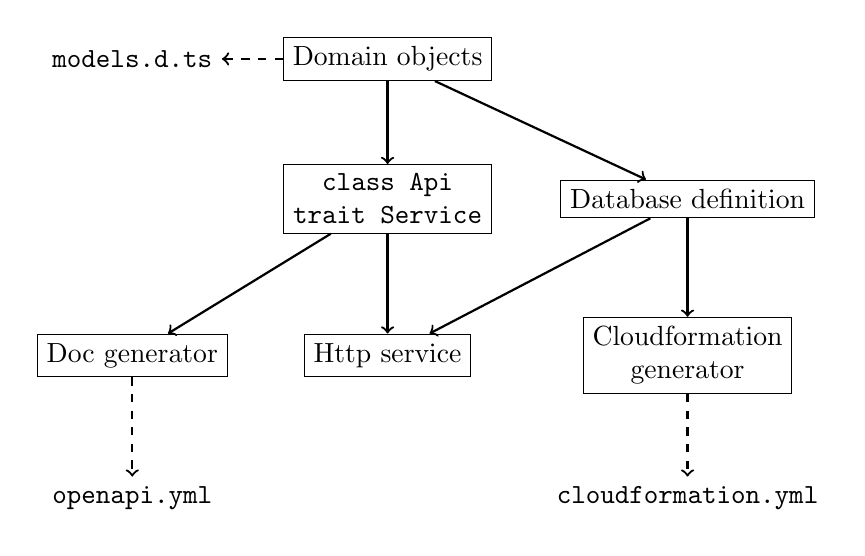
\begin{tikzpicture}[every text node part/.style={align=center}]
  \matrix [row sep=3em,
    column sep=2em]{
  \node (ts) [draw=none] {\texttt{models.d.ts}};
 & \node (src0) [draw, shape=rectangle] {Domain objects}; \\
  &  \node (src1) [draw, shape=rectangle] {\texttt{class Api} \\ \texttt{trait Service}};
 & \node(db) [draw, shape=rectangle] {Database definition}; \\
  \node (dst1) [draw, shape=rectangle] {Doc generator}; &
  \node (dst2) [draw, shape=rectangle] {Http service}; &
  \node (cfgen) [draw,shape=rectangle] {Cloudformation \\ generator}; \\
  \node (doc) [draw=none] {\texttt{openapi.yml}}; & & 
  \node (cf) [draw=none,shape=rectangle] {\texttt{cloudformation.yml}};\\} ;
  \draw[->, thick] (src1) -- (dst1);
\draw[->, thick] (src1) -- (dst2);
\draw[->, thick] (src0) -- (src1);
\draw[->,thick,dashed] (dst1) -- (doc);
\draw[->, thick, dashed] (src0) -- (ts);
\draw[->,thick] (src0) -- (db);
\draw[->,thick] (db) -- (dst2);
\draw[->,thick,dashed] (cfgen) -- (cf);
\draw[->,thick] (db) -- (cfgen);
\end{tikzpicture}
\end{frame}

\begin{frame}
\frametitle{Back to the real world}

5 questions:\pause
\begin{itemize}
\item Do you have a shared domain model between your services? \pause
\item Do you generate documentation? \pause
\item Do you generate infrastructure code? \pause
\item When adding one field to a case class, how many changed lines does your Git commit have? (including tests, etc.) \pause
\item Do you always solve problems where they occur? \pause Even if that is in an external (open source) library?
\end{itemize}


\end{frame}



\end{document}